\documentclass[8pt]{beamer}

\mode<presentation>
{
  \usetheme{AnnArbor}
  \usecolortheme{beaver}
  \usefonttheme{default}
  \setbeamertemplate{caption}[numbered]
  \setbeamercovered{transparent}
  \usefonttheme[onlymath]{serif}
  \setbeamertemplate{itemize items}[default]
  \setbeamertemplate{navigation symbols}{\insertslidenavigationsymbol\insertframenavigationsymbol}
} 

\usepackage[english]{babel}
\usepackage[utf8x]{inputenc}
\usepackage{mathtools, xcolor, soul, amsfonts, appendixnumberbeamer, graphicx, tikz}
\usepackage[makeroom]{cancel}
\graphicspath{ {images/} }

%\hypersetup{pdfpagemode=FullScreen}

\title[\scalebox{.8}{Dynamics, Simulation and Control of Quadcopters}]{Dynamics, Simulation and Control of Quadcopters}
\author[\scalebox{.8}{Dariush Hasanpoor}]{Dariush Hasanpoor}
\institute[]{Isfahan University Of Technology}
\date[\scalebox{.8}{Isfahan University Of Technology}]{Sep. 30 2015}

\newcommand{\Xtri}{$\blacktriangleright$ }
\newcommand{\Ytri}{$\triangleright$ }
\newcommand{\itemXtri}{\item[\Xtri]}
\newcommand{\itemYtri}{\item[\Ytri]}
\renewcommand{\|}[1][.3em]{\hspace{#1}|\hspace{#1}}
\renewcommand{\,}[1][.3em]{,\hspace{#1}}
\newcommand\Wider[2][3em]{%
\makebox[\linewidth][c]{\begin{minipage}{\dimexpr\textwidth+#1\relax}\raggedright#2\end{minipage}}}
\newcommand*{\Scale}[2][4]{\scalebox{#1}{$#2$}}%
\DeclarePairedDelimiter\abs{\lvert}{\rvert}%
\makeatletter
\let\oldabs\abs
\def\abs{\@ifstar{\oldabs}{\oldabs*}}
\makeatother

\definecolor{light-blue}{HTML}{66AFE9}
\definecolor{light-red}{HTML}{F77B7B}
\definecolor{light-green}{HTML}{87D13E}

\newcommand{\subitem}{\item[\Ytri]}

\begin{document}

\begin{frame}
  \titlepage
\end{frame}

\begin{frame}{Outline}
  \tableofcontents[hideallsubsections]
\end{frame}

\section{Introduction}
\frame{\tableofcontents[currentsection]}

\begin{frame}{What is a Copter?}
    \begin{itemize}[<+->]
    \item Copters are flying vehicles which use rapidly spinning rotors make themselves aloft.
    \item Conventional copters have two rotors.
    \item There are two ways that rotors can be arranged:
    \item[] \begin{itemize}
        \subitem \scalebox{0.95}{As two coplanar rotors, spinning in opposite directions.}
        \subitem \scalebox{0.95}{One main rotor providing thrust and a smaller side rotor oriented laterally.}
    \end{itemize}
    \item The design of copters comes with a control and swashplate mechanism complication.
    \item The swashplate mechanism was needed to allow the copter to utilize more degrees of freedom.
    \end{itemize}
\end{frame}

\begin{frame}{Definitions}
    \begin{block}{Degrees of Freedom (DOF)}
	DOF of a mechanical system is the number of independent parameters that define its configuration.
    \end{block}
\end{frame}

\begin{frame}{What is a Quadcopter?}
    \begin{itemize}[<+->]
    \item A quadcopter(quadrotor) is a copter which has four equally spaced rotors.
    \item With four independent rotors, the need for a swashplate mechanism is alleviated.
    \item Quadcopters can obtain copters's degrees of freedom by having two more rotors instead of swashplate.
    \item Quadcopter control is a fundamentally difficult and interesting problem due to six DOF and only four independent inputs.
    \item In order to achieve six DOF, rotational and translational motion are coupled.
    \end{itemize}
	\begin{tikzpicture}[remember picture,overlay]
	    \node at (10.8,-.7) {
	        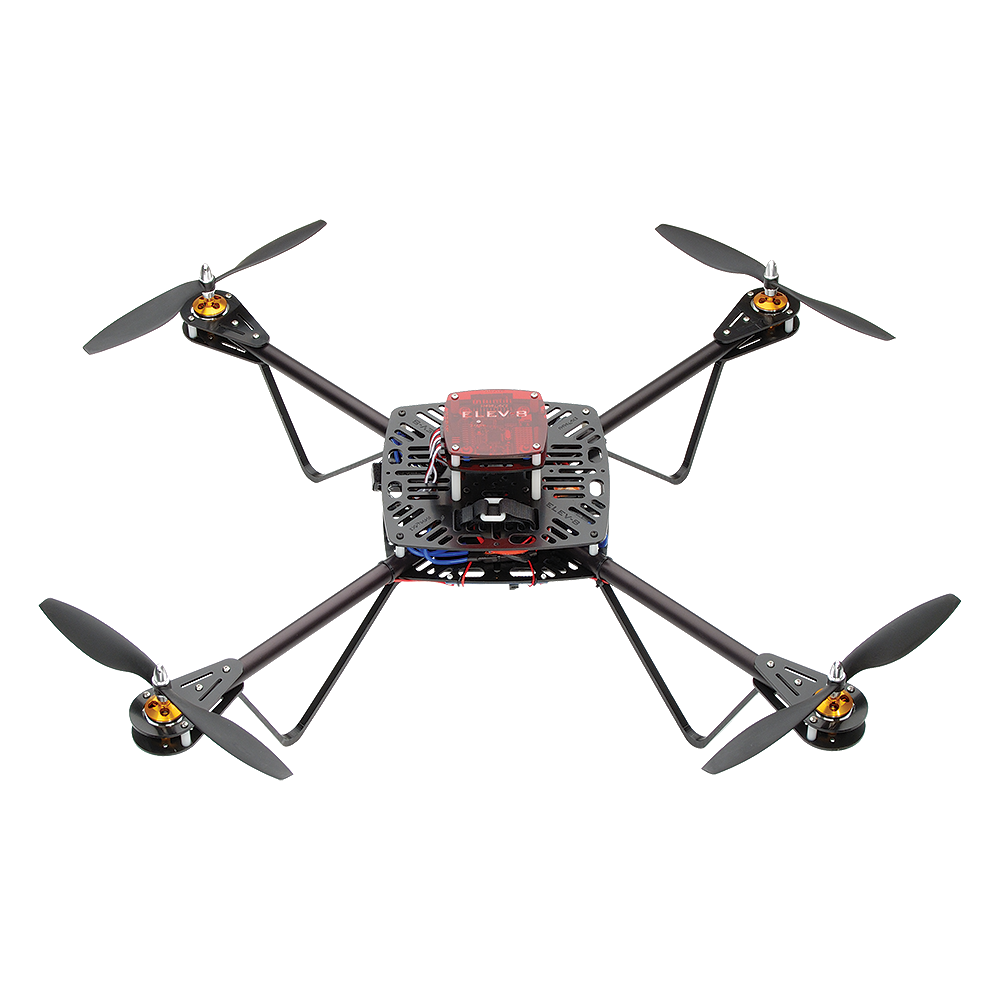
\includegraphics[width=3cm]{quadrotor}
	    };
	\end{tikzpicture}
\end{frame}

\section{Quadcopter Dynamics}
\frame{\tableofcontents[currentsection]}

\subsection{Definitions}
\begin{frame}{The Body and Inertial Frame}
    \begin{itemize}[<+->]
   \item The inertial frame is defined by the ground, with gravity pointing in the negative z direction.
    \item The body frame is defined by the orientation of the quadcopter, with the rotor axes pointing in the positive z direction and the arms pointing in the x and y directions.
    \end{itemize}
	\begin{tikzpicture}[remember picture,overlay]
	    \node at (8.8,-1.8) {
	        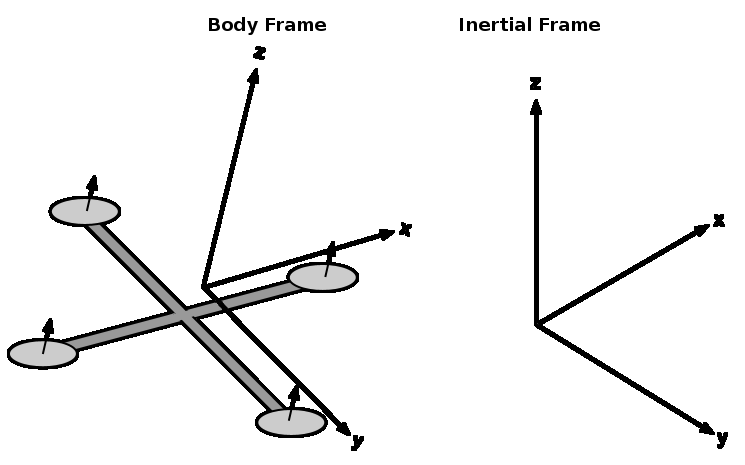
\includegraphics[width=5cm]{frames}
	    };
	\end{tikzpicture}
\end{frame}

\begin{frame}{Roll, Pitch and Yaw degrees}
    \begin{itemize}%[<+->]
    \item {\small The \textbf{roll axis} (or longitudinal axis) passes through the plane from nose to tail -- alongside of $x$ axis.}
    \item {\small The \textbf{pitch axis} (also called lateral or transverse axis) passes through the plane from wingtip to wingtip -- alongside of $y$ axis.}
    \item {\small The vertical \textbf{yaw axis} is defined to be perpendicular to the wings with its origin at the center of gravity and directed towards the bottom of the aircraft -- alongside of $z$ axis.}
    \end{itemize}
	\begin{tikzpicture}[remember picture,overlay]
	    \node at (9,-1.75) {
	        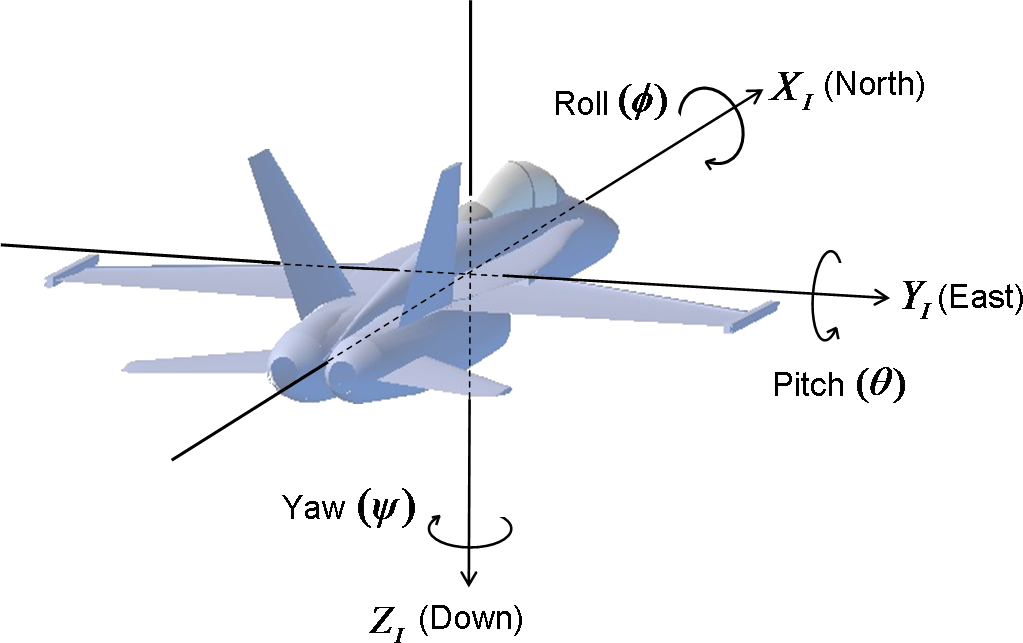
\includegraphics[width=5cm]{roll-pitch-yaw}
	    };
	\end{tikzpicture}
\end{frame}

\subsection{Kinematics}
\begin{frame}{Basics of The Kinematic}
    \begin{itemize}[<+->]
    \item Position and velocity of the quadcopter in the inertial frame are defined as $p = (x, y, z)^T$ and $\dot{p} = (\dot{x}, \dot{y}, \dot{z})^T$, respectively.
    \item The roll, pitch, and yaw angles in the body frame are defined as $\theta = (\phi, \theta, \psi)^T$, with corresponding angular velocities equal to $\dot{\theta} = (\dot{\phi}, \dot{\theta}, \dot{\psi})^T$.
    \end{itemize}
\end{frame}

\begin{frame}{Basics of The Kinematic}{cont.}
    \begin{itemize}[<+->]
    \item In order to convert roll, pitch and yaw velocities into the angular velocity vector, we can use the following relation:
    \item[] \begin{equation}
    \omega = \begin{bmatrix}
    1 & 0 & -s_\theta\\
    0 & c_\phi & s_{\theta}s_\phi\\
    0 & -s_\phi & c_{\theta}c_\phi
    \end{bmatrix} \dot{\theta}
    \end{equation}\\ where $\omega$ is the angular velocity vector in the body frame.
    \end{itemize}
\end{frame}

\begin{frame}{Basics of The Kinematic}{cont.}
    \begin{itemize}[<+->]
    \item Rotation matrix $R$ relates the body and inertial frame, which goes from the body frame to the inertial frame.
    \item[] \begin{equation}
    R = \begin{bmatrix}
    c_{\phi}c_{\psi} - c_{\theta}s_{\phi}s_{\psi} & -(c_{\psi}s_{\phi} + c_{\phi}c_{\theta}s_{\psi}) & s_{\theta}s_{\psi}\\
    c_{\theta}c_{\psi}s_{\phi} + c_{\phi}s_{\psi} & c_{\phi}c_{\theta}c_{\psi} - s_{\phi}s_{\psi} & -c_{\psi}s_{\theta}\\
    s_{\phi}s_{\theta} & c_{\phi}s_{\theta} & c_{\theta}
    \end{bmatrix}
    \end{equation}
    \item This matrix is derived by using the \textit{ZYZ Euler angle} conventions.
    \item For a given vector $\vec{v}$ in the body frame, the corresponding vector is given by $R\vec{v}$ in the inertial frame.
    \end{itemize}
\end{frame}

\begin{frame}{Physics}
    \begin{itemize}%[<+->]
    \item In order to properly model the dynamics of the system, we need an understanding of the physical properties that govern it.
    \item Topics which are going to discuss in this section are as follow:
    \item[] \begin{itemize}
        \subitem Motors
        \subitem Forces
        \subitem Torques
    \end{itemize}
    \end{itemize}
\end{frame}

\begin{frame}{Physics}{Motors}
    \begin{itemize}
    \item For electric motors, the torque produced is given by:
    \item[] \begin{equation}
    \tau = K_t(I-I_0)
    \end{equation}
    \pause
    \item Where:
    \begin{itemize}
        \subitem $\tau$ is the motor torque.
        \subitem $I$ is the input current.
        \subitem $I_0$ is the current when there is no load on the motor.
        \subitem $K_t$ is the torque proportionality constant.
    \end{itemize}
    \end{itemize}
\end{frame}

\begin{frame}{Physics}{Motors -- cont.}
    \begin{itemize}
    \item The voltage across the motor is:
    \item[] \begin{equation}
    V = IR_m + K_v\omega
    \end{equation}
    \pause
    \item Where:
    \item[] \begin{itemize}
        \subitem $V$ is the voltage drop across the motor.
        \subitem $R_m$ is the motor resistance.
        \subitem $\omega$ is the angular velocity of the motor.
        \subitem $K_v$ is a proportionality constant.
    \end{itemize}
    \end{itemize}
\end{frame}

\begin{frame}{Physics}{Motors -- cont.}
    \begin{itemize}
    \item The motor's power consumption is:
    \item[] \begin{equation}
    P = IV = \frac{(\tau + K_tI_0)(K_tI_0R_m + {\tau}R_m + K_tK_v\omega)}{K_t^2}
    \end{equation}
    \pause
    \item For the purposes of our simple model, we will assume:
    \item[] \begin{itemize}
        \subitem A negligible motor resistance(i.e $R_m \approx 0$).
        \subitem $K_tI_0 \ll \tau$
    \end{itemize}
    \item[] \vspace{-2.5em}\begin{align}
    P = IV  &= \frac{(\tau + K_tI_0)(\cancelto{0}{K_tI_0R_m} + \cancelto{0}{{\tau}R_m} + K_tK_v\omega)}{K_t^2}\nonumber\\
            &= \frac{\cancelto{\tau}{(\tau + K_tI_0)}K_v\omega}{K_t}\nonumber\\
            &= {K_v \over K_t}\tau\omega\label{eq:PTW}
    \end{align}
    \end{itemize}
\end{frame}


\begin{frame}{Physics}{Forces}
    \begin{itemize}
    \item  By conservation of energy, we know that:
%   (energy the motor expends) X (in a given time period) == (the force generated on the propeller) X (the distance that the air it displaces moves)
    \item[]\hspace{1em}\begin{equation}
    P.dt = F.dx
    \end{equation}
    \pause
    \item Equivalently, the power is equal to the thrust times the air velocity:
    \item[] \begin{equation}
    F = {P \over v_h} \xRightarrow{\text{eq.\ref{eq:PTW}}} F = { K_p\tau\omega \over v_h}
    \label{eq:motors_force}
    \end{equation}
    \pause
    \item We assume that:
    \item[] \begin{itemize}
        \subitem Vehicle speeds are low, so $v_h$ is the air velocity when hovering.
        \subitem The free stream velocity, $v_{\infty}$ is zero.
        \subitem Since $v_{\infty} = 0$ this is obvious that $v_h \sim  K_mv_m$.
        % ^ the air in the surrounding environment is stationary relative to the quadcopter.
    \end{itemize}
    \end{itemize}
\end{frame}

\begin{frame}{Physics}{Forces -- cont.}
    \begin{itemize}
    \item As torque is defined in The aerodynamic drag, we have:
    \item[] \begin{equation}
    \tau = {1 \over 2}{\rho}Av_{h}^2
    \label{eq:torque}
    \end{equation}
    \pause
    \item Where:
    \item[] \begin{itemize}
        \subitem $\rho$ is the density of the surrounding air.
        \subitem $A$ is the area swept out by the rotor.
    \end{itemize}
    \pause
    \item From equations \ref{eq:motors_force} and \ref{eq:torque}, we can derive the following equation:
    \item[] \begin{align*}
    F &= { K_p\tau\omega \over v_m}\\
      &\stackrel{\text{eq.\ref{eq:torque}}}{=\joinrel=} {K_p \over 2}{\rho}Av_{m}\omega
    \end{align*}
    \pause
    \begin{equation}
    F = T \xRightarrow{\omega = {v_m \over r}} T = k\omega^2
    \label{eq:thrust}
    \end{equation}
    \end{itemize}
\end{frame}

\begin{frame}{Physics}{Forces -- cont.}
    \begin{itemize}
    \item By eq.\ref{eq:thrust} total thrust on the quadcopter(in the body frame) is given by:
    \item[] \begin{equation}
    T_B = \sum_{i = 1}^4 T_i = k\begin{bmatrix}
    0\\0\\\sum_{i = 1}^4w_i
    \end{bmatrix}
    \end{equation}
    \pause
    \item For modeling the friction, we will assume highly simplified version, which is:
    \item[] \begin{equation}
    F_D = -k_d\begin{bmatrix}
    \dot{x}\\\dot{y}\\\dot{z}
    \end{bmatrix}     
    \end{equation}
    \end{itemize}
\end{frame}

\begin{frame}{Physics}{Torques}
    \begin{itemize}[<+->]
    \item Each rotor contributes some torque about the body z axis.
    \item The torque is required to keep the propeller spinning and providing thrust.
    \item It creates the instantaneous angular acceleration and overcomes the frictional drag forces.
    \item The drag equation from fluid dynamics gives us the frictional force:
    \item[] \begin{equation}
    F_D = {1 \over 2}{\rho}C_DAv^2
    \label{eq:drag_force}
    \end{equation}
    \item Where:
    \item[] \begin{itemize}
        \subitem $\rho$ is the surrounding fluid density.
        \subitem $A$ is the reference area.
        \subitem $C_D$ is a dimensionless constant.
    \end{itemize}
    \end{itemize}
\end{frame}

\begin{frame}{Physics}{Torques -- cont.}
    \begin{itemize}
    \item In general cases torque is cross product of distance vector and the applied force:
    \item[] \begin{equation}
    \tau = \vec{r} \times \vec{F}
    \label{eq:torque_in_general}
    \end{equation}
    \only<2->{\item From eq.\ref{eq:drag_force} and eq.\ref{eq:torque_in_general} we have:
    \item[] \begin{equation}
    \tau_D = {1 \over 2}R{\rho}C_DAv^2 \xRightarrow{\omega = {v \over R}} \tau_D = {1 \over 2}R{\rho}C_DA(R\omega)^2 = b\omega^2
    \label{eq:torque_drag}
    \end{equation}}
    \only<2>{\item Where:
    \item[] \begin{itemize}
        \subitem $\omega$ is the angular velocity of the propeller.
        \subitem $R$ is the radius of the propeller.
    \end{itemize}}
    \end{itemize}
    \only<3>{\begin{block}{Note:}
    We've assumed that all the force is applied at \textbf{the tip of the propeller}, which is certainly \underline{inaccurate}.
    \end{block}}
\end{frame}

\begin{frame}{Physics}{Torques -- cont.}
    \begin{itemize}
    \item Torque about the z-axies for the $i$th motor is eqaul to:
    \item[] \begin{equation}
    \tau_i^z = \tau_{D_i} + I_M\dot{\omega}_i = b\omega_i^2 + I_M\dot{\omega}_i
    \label{eq:torque_about_zaxis}
    \end{equation}
    \pause
    \item Where:
    \item[] \begin{itemize}
        \subitem $I_M$ is the moment of inertia about the motor z-axis.
        \subitem $\dot{\omega}$ is the angular acceleration of the propeller.
        \subitem $b$ drag coefficient constant.
    \end{itemize}
    \pause
    \item Note that in eq.\ref{eq:torque_about_zaxis} in steady state flight, $\dot{\omega}_i \approx 0$. So for simplification of our model we will assume $I_M\dot{\omega}_i = 0$.
    \pause
    \item Inorder to neutralize the overall torque in quadcopter steady-state, two of the motors should spin clockwise, and the other two should spin counter-clockwise.
    \end{itemize}
\end{frame}

\begin{frame}{Physics}{Torques -- cont.}
    \begin{itemize}
    \item Eq.\ref{eq:torque_about_zaxis} can be written as following for each propellor:
    \item[] \begin{equation}
    \tau_i^z = (-1)^{i+1}b\omega_i^2
    \end{equation}
    \item Which the $(-1)^{i+1}$ term is positive for the ith propeller if the propeller is spinning clockwise and negative if it is spinning counterclockwise.
    \pause
    \item The total torque about the axises can be derived from standard mechanics:
    \item[] \begin{align}
    &\tau_\psi = b\sum_{i=1}^4 (-1)^{i+1}\omega_i^2\label{eq:total_torque_z}\\
    &\tau_\theta = \sum_{i \in \{2, 4\}} \vec{r} \times T = Lk(\omega_2^2 - \omega_4^2)\label{eq:total_torque_y}\\
    &\tau_\phi = \sum_{i \in \{1, 3\}} \vec{r} \times T = Lk(\omega_1^2 - \omega_3^2)\label{eq:total_torque_x}
    \end{align}
    \item Where the $L$ is the distance from the center of the quadcopter to any of the propellers.
    \end{itemize}
\end{frame}

\begin{frame}{Physics}{Torques -- cont.}
    \begin{itemize}
    \item From equations \ref{eq:total_torque_z}\ldots\ref{eq:total_torque_x} we can calculate the torque matrix in body frame:
    \item[] \begin{equation}
    \tau_B = \begin{bmatrix}
    Lk(\omega_1^2 - \omega_3^2)\\\\
    Lk(\omega_2^2 - \omega_4^2)\\\\
    b\sum_{i=1}^4 (-1)^{i+1}\omega_i^2
    \end{bmatrix}
    \end{equation}
    \end{itemize}
\end{frame}

\begin{frame}{Physics}{What we have ignored in our modelings?}
    \begin{itemize}[<+->]
    \item Rotational drag forces(our rotational velocities are relatively low).
    \item Blade flapping(deformation of propeller blades due to high velocities and flexible materials).
    \item Surrounding fluid velocities(wind).
    \item The noise distribution model of our motors' speed.
    \item etc.
    \end{itemize}
\end{frame}

\begin{frame}{Equations of Motion}{Acceleration}
    \begin{itemize}%[<+->]
    \item In the inertial frame, the acceleration of the quadcopter is due to thrust, gravity and linear friction.
    \item We can obtain the thrust vector in the inertial frame by using the rotation matrix $R$ to map the thrust vector from the body frame to the inertial frame:
    \item[] \begin{align}
    &F = m\ddot{x}\\
    &F = m\vec{G} + RT_B + F_D\\
    &\ddot{x} = \begin{bmatrix}
    0\\0\\-g
    \end{bmatrix} + {{RT_B + F_D} \over m}
    \end{align}
    \item Where:
    \item[] \begin{itemize}
        \subitem $\vec{x}$ is the position of the quadcopter.
        \subitem $g$ is the acceleration due to gravity.
        \subitem $F_D$ is the drag force.
        \subitem $T_B$ is the thrust vector in the body frame.
    \end{itemize}
    \end{itemize}
\end{frame}

\begin{frame}{Equations of Motion}{Rotational Speed -- cont.}
    \begin{itemize}%[<+->]
    \item Rotational equations can be drived from Euler's equations for rigid body dynamics, Expressed in vector form:
    \item[] \begin{equation}
    I\dot{\omega} + \omega \times (I\omega) = \tau
    \label{eq:euler-rot-eq}
    \end{equation}
    \item Where:
    \item[] \begin{itemize}
        \subitem $\omega$ is the angular velocity vector.
        \subitem $I$ is the inertia matrix.
        \subitem $\tau$ is a vector of external torques.
        \subitem $T_B$ is the thrust vector in the body frame.
    \end{itemize}
    \item The eq.\ref{eq:euler-rot-eq} can rewrite this as:
    \item[] \begin{equation}
    \dot{\omega} = \begin{bmatrix}
    \dot{\omega}_x\\\dot{\omega}_y\\\dot{\omega}_z
    \end{bmatrix} = I^{-1}(\tau - \omega\times(I\omega))
    \end{equation}
    \end{itemize}
\end{frame}

\begin{frame}{Equations of Motion}{Rotational Speed -- cont.}
    \begin{itemize}%[<+->]
    \item For simplification if we assume that the quadcopter as two thin uniform rods crossed at the origin with a point mass (motor) at the end of each; The inertia matrix would come in form of a diagonal matrix.
    \item[] \begin{equation}
    I = \begin{bmatrix}
    I_{xx}&0&0\\
    0&I_{yy}&0\\
    0&0&I_{zz}
    \end{bmatrix}
    \end{equation}
    \item Therefore, we obtain our final result for the body frame rotational equations of motion:
    \item[] \begin{equation}
    \dot{\omega} = \begin{bmatrix}
    \tau_{\phi}I_{xx}^{-1}\\
    \tau_{\theta}I_{yy}^{-1}\\
    \tau_{\psi}I_{zz}^{-1}
    \end{bmatrix} - \begin{bmatrix}
    {{I_{yy} - I_{zz}} \over I_{xx}}\omega_y\omega_z\\
    {{I_{zz} - I_{xx}} \over I_{yy}}\omega_x\omega_z\\
    {{I_{xx} - I_{yy}} \over I_{zz}}\omega_x\omega_y
    \end{bmatrix}
    \end{equation}
    \end{itemize}
\end{frame}
\section{References}
\begin{frame}{References}
    \nocite{*}
    {\scriptsize
    \begin{thebibliography}{1}
    \bibitem{}
    L. R. Garcia Carrillo, A. E. Dzul Lopez, R. Lozano, and C. Pegard, "Introduction," in Quad Rotorcraft Control, London: Springer London, 2013, pp. 1–22.
    \bibitem{}
    L. R. Garcia Carrillo, A. E. Dzul Lopez, R. Lozano, and C. Pegard, "Modeling the Quad-Rotor Mini-Rotorcraft," in Quad Rotorcraft Control, London: Springer London, 2013, pp. 23–34.
    \bibitem{}
    N. Sydney, B. Smyth, D. Paley, and others, "Dynamic control of autonomous quadrotor flight in an estimated wind field," in Decision and Control (CDC), 2013 IEEE 52nd Annual Conference on, 2013, pp. 3609–3616.
    \bibitem{}
    S. L. Waslander and C. Wang, "Wind disturbance estimation and rejection for quadrotor position control," in AIAA Infotech@ Aerospace Conference and AIAA Unmanned... Unlimited Conference, Seattle, WA, 2009.
    \bibitem{}
    E. B. Nice, "Design of a four rotor hovering vehicle," Cornell University, 2004.
    \end{thebibliography}
    }
\end{frame}

\appendix

\end{document}